\documentclass[10pt]{beamer}


\usepackage[utf8]{inputenc}
\usepackage[brazil]{babel}
\usepackage{graphicx}		% utilizado para inserir gráfico

% Usado para incluir código
\usepackage{listings}
% Needed to use citations.
\usepackage{cite}

\usetheme{Copenhagen}
\usecolortheme{lccv}
\setbeamertemplate{background}{
\includegraphics[width=\paperwidth]{./figuras/background_lccv.jpg}}
%\setbeamercovered{transparent}

\title[]{\textbf{Cloud} e \textbf{Grid}: Quais as diferenças?}
\author[]{Baltazar Tavares Vanderlei}
\date{15 de março de 2013}
\institute[2013]{Laboratório de Computação Científica e Visualização - LCCV/UFAL}

\begin{document}

\newcommand{\til}{\~{}}

\frame{\titlepage}
	\begin{frame}[t]
	\frametitle{Sumário}
	\tableofcontents[framebreaks]
	%\tableofcontents[pausesections]
\end{frame}

% Perfumaria sobre o sumário ser mostrado a cada passagem de sessão e sub-sessão.
\AtBeginSection[]{
	\begin{frame}[t]
	\frametitle{Sumário}
	\tableofcontents[currentsection]
	\end{frame}
}

\AtBeginSubsection[]{
	\begin{frame}[t]
	\frametitle{Sumário}
	\tableofcontents[currentsubsection]
	\end{frame}
}

\section{Introdução}
	\begin{frame}%[t]
	\frametitle{Classificando pelo tipo de serviço}
		\text{Para o serviço disponibilizado, podemos classifica-lo como:}
		\begin{itemize}%[<+->]
			\item \textbf{\textbf{SaaS}}: Software as a Service
			\begin{itemize}
				\item \textbf{skype, GMail, facebook} ...
			\end{itemize}
			\item \textbf{\textbf{PaaS}}: Plataform as a Service
			\begin{itemize}
				\item \textbf{Wordpress, Freezope, Openshift} ...
			\end{itemize}
			\item \textbf{\textbf{IaaS}}: Infrastructure as a Service
			\begin{itemize}
				\item \textbf{Amazom, \textbf{Nimbus}, \textbf{OpenStack}} ...
			\end{itemize}
		\end{itemize}
		\pause
		\begin{block}{OBS:}
			O \textbf{IaaS} popularizou mais com o surgimento de tecnologias de virtualização
		\end{block}
	\end{frame}

	\begin{frame}%[t]
	\frametitle{Comparando tudo}
		\begin{figure}
		\centering
			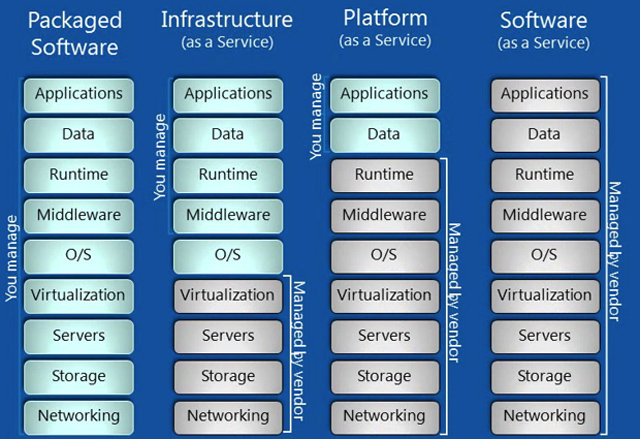
\includegraphics[scale=0.4]{./figuras/iaas-paas-saas.jpg}
%			\caption{Resumão: \textbf{IaaS}, \textbf{PaaS}, \textbf{SaaS}, EaaS, MaaS...}
		\end{figure}
	\end{frame}

\section{Grid}
	\subsection{Características}

		\begin{frame}
		\frametitle{Que caracteriza um grid?}
			\begin{block}{Segundo \textbf{Ian Foster}:}
			% http://dlib.cs.odu.edu/WhatIsTheGrid.pdf
			\begin{itemize}
				\item ...coordinates resources that are not subject to centralized control...
				\item ...using standard, open, general-purpose protocols and interfaces...
				\item ...to deliver nontrivial qualities of service.
			\end{itemize}
			\end{block}
			\begin{block}{Segundo \textbf{Buyya/Venugopal}:}
				a type of parallel and distributed system that enables the sharing, selection, and aggregation of geographically distributed autonomous resources dynamically at runtime depending on their availability, capability, performance, cost, and users quality-of-service requirements
			\end{block}
		\end{frame}

		\begin{frame}%[t]
		\frametitle{Podemos ressaltar:}
			\begin{itemize}%[<-+>]
				\item Colaboração
				\item Padrões
				\begin{itemize}%[<-+>]
					\item \textbf{JSDL}
					\item \textbf{Web Services}
				\end{itemize}
				\item Organização de recursos
				\item Acadêmico, bem mais definido
				\item Perfil de aplicação voltado para batch( não exclusivo )
				\item Surgiu antes de virtualização se consolidar
			\end{itemize}
		\end{frame}

	\subsection{Projetos}

		\begin{frame}%[t]
			\begin{itemize}%[<-+>]
				\item OurGrid
				\item SETI@home
				\item Globus Toolkit
				\item Muitos outros projetos academicos
			\end{itemize}
		\end{frame}

\section{Cloud}
	\subsection{Características}

		\begin{frame}
		\frametitle{Que caracteriza uma Cloud?}
			% http://venturebeat.com/2011/11/14/cloud-iaas-paas-saas/
			\begin{block}{Segundo \textbf{Sean Ludwig}:}
				Let’s start at the beginning. “Cloud” is a metaphor for the Internet, and “cloud computing” is using the Internet to access applications, data or services that are stored or running on remote servers.
\newline
\newline
				When you break it down, any company offering an Internet-based approach to computing, storage and development can technically be called a cloud company. However, not all cloud companies are the same. Typically, these companies focus on offering one of three categories of cloud computing services. These different segments are called the “layers” of the cloud.
			\end{block}
		\end{frame}

		\begin{frame}%[t]
		\frametitle{Podemos ressaltar:}
			\begin{itemize}%[<-+>]
				\item Voltado a serviços: \textbf{IaaS}, \textbf{PaaS}, \textbf{SaaS} ...
				\item Mais usado da industria, bem menos definido
				\item Pay-as-you-go (on demand) ?
				\item Recursos infinitos e elasticos ?
				\item Sem padrões bem definidos
				\item Virtualização bem mais usada
			\end{itemize}
		\end{frame}

	\subsection{Projetos}

		\begin{frame}%[t]
			\begin{itemize}%[<-+>]
				\item \textbf{Nimbus}
				\item \textbf{OpenStack}
				\item \textbf{OpenNebula}
				\item \textbf{Amazon}
			\end{itemize}
		\end{frame}

\section{Comparando}
	\begin{frame}%[t]
	\begin{block}{Cloud}
		\begin{itemize}%[<-+>]
			\item Usa muito como padrão o \textbf{Amazon}
			\item Mais integrada a virtualização
			\item Voltado a industria, a venda de serviço, de apenas uma organização
			\item Começou pensando em \textbf{IaaS}, pode suportar \textbf{PaaS} e \textbf{SaaS}
			\item Emgloba grid, por ser muito generico
		\end{itemize}
	\end{block}

	\begin{block}{Grid}
		\begin{itemize}%[<-+>]
			\item Padrões bem mais definidos, por isso subconjunto de cloud
			\item Menos integrado a virtualização, mas presente
			\item Mais de origem academica, a gerenciar recursos compartilhados, multi-institucional
			\item Começou pensando em \textbf{PaaS} e \textbf{SaaS}, pode suportar \textbf{IaaS}
		\end{itemize}
	\end{block}
	\end{frame}

	\begin{frame}%[t]
	\frametitle{Cloud vs Grid: Questão de ponto de vista}
		\begin{figure}
		\centering
			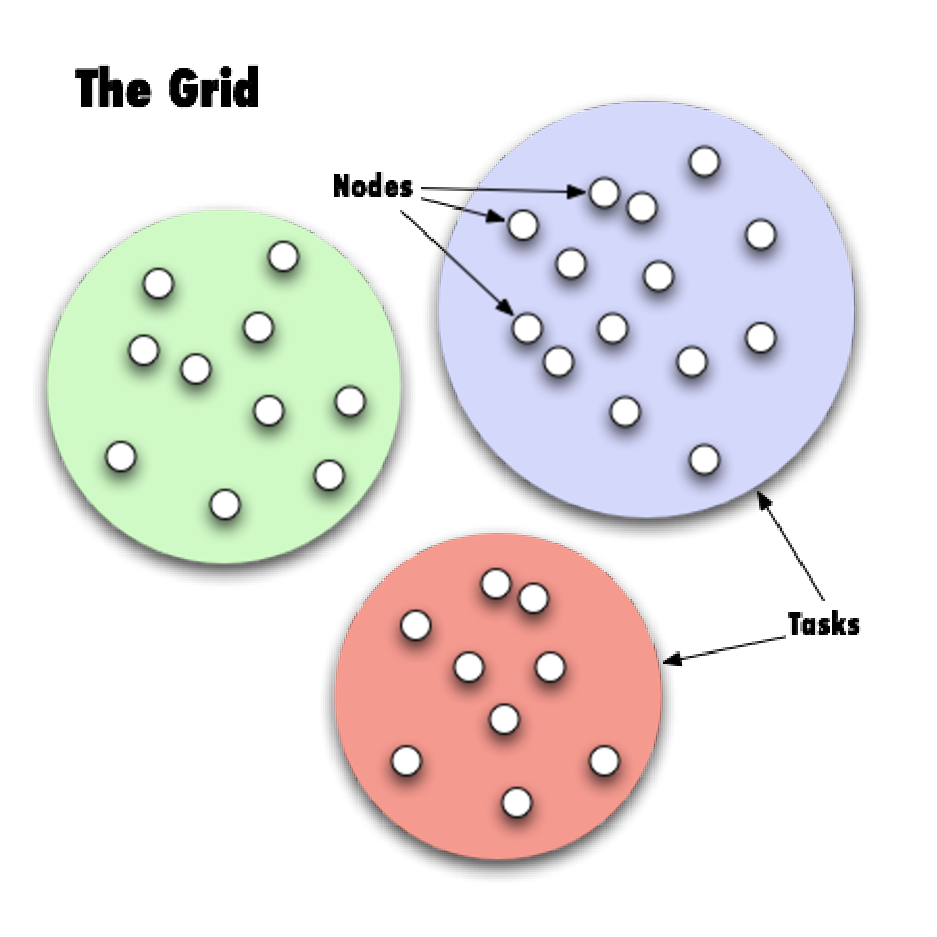
\includegraphics[scale=0.29]{./figuras/grid-nodes.pdf}
			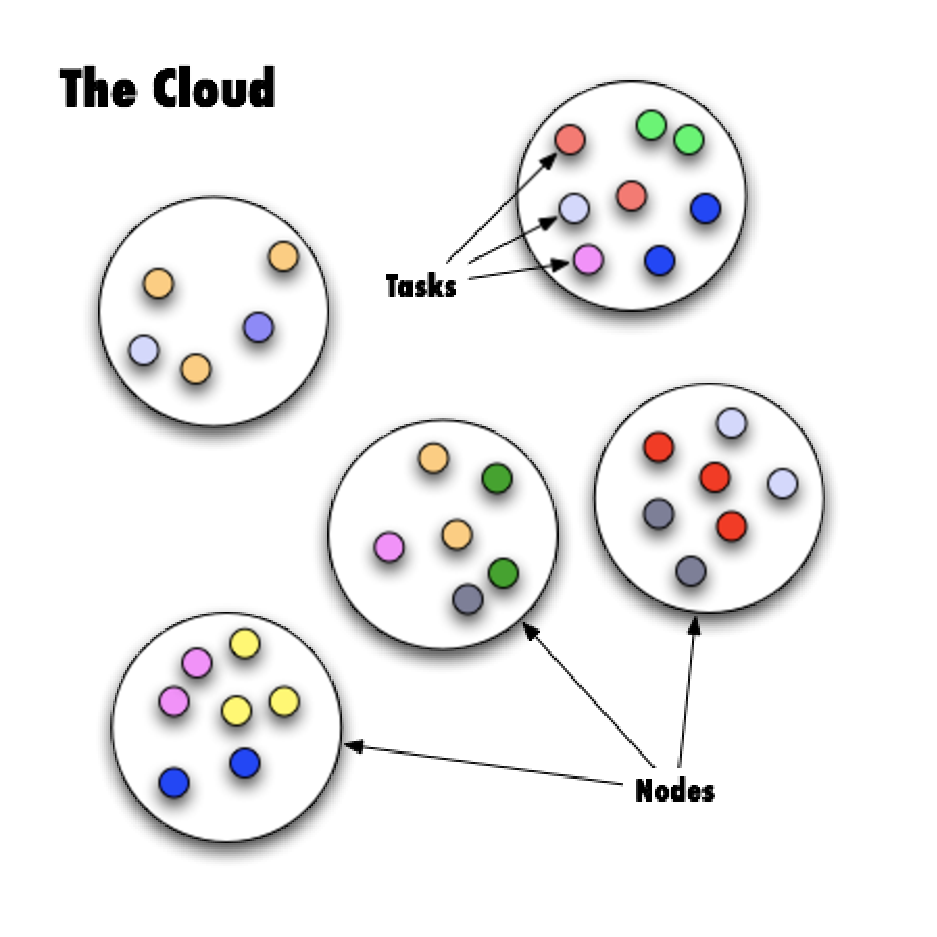
\includegraphics[scale=0.29]{./figuras/cloud-nodes.pdf}
		\end{figure}
	\end{frame}





%%\section{Refs}
%%	\begin{frame}%[t]
%%	\frametitle{Vamos comparar os grafos...}
%%		\bibliography{Refs}{}
%%		\bibliographystyle{plain}
%%	\end{frame}


%%%%%%%%%%%% End
\begin{frame}%[t]
\frametitle{\centering Fim!}
	\begin{figure}
	\centering
		
\includegraphics[scale=2]{./figuras/cloud_oops.jpg}
	\end{figure}
\end{frame}
\end{document}

% http://www.slideshare.net/rsmontero/cloud-and-grids

